\subsection{Lautstärkeverarbeitung}\label{subsec:Volume_Generation}
Die Aufgabe der \textit{Lautstärkenverarbeitung} ist es aus dem Signal des Lautstärkenoszillators einen Dämpfungsfaktor zu berechnen, mit welchem das Signal der Tonhöhenverarbeitung multipliziert wird. So kann der Spieler die Lautstärke während dem Spielen wie die Tonhöhe über eine Antenne einstellen. Wie Abbildung \ref{img:Blockschaltbild_volume} zeigt sind die beiden Verarbeitungskomponenten auch sehr ähnlich. Der Referenzoszillator und der Mischer sind gleich wie in der Tonverarbeitung. In den nächsten Abschnitten sind die Unterschiede zu den Komponenten der Tonverarbeitung aufgezeigt.



\begin{figure}[h!]
	\centering
	\includegraphics[width=1\textwidth]{Blockschaltbild_Volume.pdf}
	\caption{Blockschaltbild der Custom IP Volume Generation} 
	\label{img:Blockschaltbild_volume}
\end{figure}  


\newpage
\paragraph{Filter}\mbox{}\\

Beim \textit{Filter} der Laustsärkeverarbeitung ist die Frequenzmessung erst nach dem dritten CIC Filter angeschlossen. Wir haben dies so entschieden, um beim FIR-Filter der Frequenzmessungskomponente weniger Koeffizienten und somit weniger Ressourcen zu benötigen. Das FIR-Filter benötigt deshalb weniger Koeffizienten, da nach CIC 3 die Abtastfrequenz des Signals um den Faktor 45 kleiner ist, nämlich 240kHz. Zudem ist das FIR-Filter in dieser Komponente deswegen nicht mehr nötig.

\begin{figure}[h!]
	\centering
	\includegraphics[width=0.8\textwidth]{Filter_volume.pdf}
	\caption{Aufbau des Filters in der Komponente Volume Generation} 
	\label{img:Filter_Volume}
\end{figure}  

\paragraph{Frequenzmessung \& Kalibration}\mbox{}\\

Auch bei der Komponente \textit{Frequenzmessung} waren Anpassungen nötig. 
Die Abtastfrequenz des Signals aus dem Filter haben wir wie im vorherigen Abschnitt besprochen auf 240kHz gesetzt. Dies bedeutet, dass die Frequenzmessung weniger genau ist, was jedoch für die Einstellung der Lautstärke nicht problematisch ist, verglichen zu der Tonhöhe. Der Vorteil von einer tieferen Abtastfrequenz ist, dass das FIR-Filter weniger Filterkoeffizienten hat und somit Ressourcen einspart.\\
Der Periodenzähler ist gleich geblieben wie in der Tonhöhenverarbeitung.\\
Anders als zuvor sind nun zwei Goldschmidtdividierer verbaut. Dies um den in Kapitel \ref{subsec:Pitch_Generation} besprochenen Dämpfungsfaktor zu berechnen und an die Tonhöhenverarbeitung weiterzugeben. Wie zuvor berechnet der \textit{Goldschmidtdividierer 1} aus der Anzahl Abtastperioden aus per\_cnt die entsprechende Frequenz. \textit{Goldschmidtdividierer 2} berechnet aus der Frequenz den erwähnten Dämpfungsfaktor. Wir haben uns dafür entschieden diese Berechnung so einzustellen, dass alle Messungen unter \SI{300}{Hz} einen Dämpfungsfaktor 0 oder kein Ton ergibt. Das Maximum oder 1 haben wir auf \SI{3500}{Hz} eingestellt. Da die Frequenz des Signals welches vom Filter kommt exponentiell ansteigt, muss keine Umrechnung stattfinden um die Eigenschaft des logarithmischen Gehörs zu kompensieren.

Anders als bei der gleichen Komponente in der Tonhöhenverarbeitung ist die Funktionalität des Glissando-Effekts in der Lautstärkeverarbeitung nicht nötig. Die Kalibration funktioniert jedoch gleich wie in der Tonhöhenverarbeitung.

\begin{figure}[h!]
	\centering
	\includegraphics[width=1\textwidth]{freq_meas_volume.pdf}
	\caption{Aufbau der Frequenzmessung und Kalibration in der Komponente Volume Generation} 
	\label{img:freq_meas_volume}
\end{figure}  

\newpage

\paragraph{Register}\mbox{}\\
Um mit der Komponente \textit{Lautstärkenverarbeitung} über das Memory-Mapped Interface kommunizieren zu können haben wir das folgende Register definiert:


\begin{table}[H]
	\centering
	\caption{Control Register Flags}
	\label{tab:Register_volume_cntrl}
	\begin{tabular}{l|l|l|l}
		\textbf{Bits} & \textbf{Kürzel} & \textbf{R/W} &	\textbf{Beschreibung}\\
		\hline \hline
		
		0 & ant\_on & W &  1 = Lautstärkeantenne aktiviert \\ 
		&      &   &  0 = Lautstärkenantenne deaktiviert \\ 
		\hline
		1 & cal & R/W &  1 = Kalibration aktiviert \\ 
		&     &     &  0 = Kalibration beendet \\ 
		\hline
	
	\end{tabular}
\end{table}

Ist das Flag ant\_on auf 0 gesetzt, lässt sich das Theremin nur über die Tonhöhenantenne spielen. Die Lautstärke ist dabei immer konstant.

